\chapter{Results}
\label{chapter:Results}

This chapter validates the cost model of
Chapter \ref{chapter:methodology} by measuring the run time, memory
traffic and scaling behaviour of the proposed
solver.  After describing the test bed and the benchmark protocol, the
observed performance is compared to Intel~MKL’s single–threaded
\texttt{d\_trsv} routine and a parallel routine based on Kokkos. In Section \ref{sec:results:cache-reuse} cache reuse and the effectiveness of the affinity clause is measured and discussed.

%--------------------------------------------------------------------
\section{Benchmark Platforms}
\label{sec:res_platforms}

All experiments were performed on two compute nodes of the DelftBlue supercomputer \cite{delftblue_system},  their most
relevant characteristics are summarised in Table \ref{tab:platforms}.  Each result section states explicitly
which platform was used.

\begin{table}[ht]
  \centering
  \caption{Hardware and software environment.}
  \label{tab:platforms}
  \begin{tabular}{lcc}
    \toprule
                    & DelftBlue (Compute-p1)    & DelftBlue (Compute-p2)  \\
    \midrule
    CPU model       & Intel Xeon E5-6248R  & Intel Xeon E5-6448Y  \\
    Micro‐architecture & Cascade Lake      &  Sapphire rapids   \\
    Cores / SMT     & 24C / 48T &  32C / 64T  T \\
    Nominal clock   & 3.0 GHz                &  2.1GHz    \\
    L3 cache        & 36 MiB                 &  60 MiB   \\
    Memory          & 185 GiB DDR4-2933      &   250 GiB DDR4-2933  \\
    Compiler        & gcc 15.1.0 & gcc 15.1.0 \\
    MKL             & oneAPI 2023.2            &   oneAPI 2023.2  \\
    LIKWID          & 5.4.1                    &  5.4.1   \\
    \bottomrule
  \end{tabular}
\end{table}

%--------------------------------------------------------------------
\section{Test Matrices}
\label{sec:res_matrices}
%--------------------------------------------------------------------
The test set comprises ten sparse matrices drawn from the SuiteSparse
collection \cite{10.1145/2049662.2049663}. The full list of the matrices used for testing is given in Table \ref{tab:matrices_benchmarks}.
Prior to factorisation each matrix is symmetrised (if necessary),
reordered by RACE, and its lower–triangular part extracted, exactly as described in Section \ref{chap:meth_problem_simp_and_reorder}.  

The benchmark uses the lower–triangular part of $A^{k}$.
Taking the cubic power is an inexpensive, purely algebraic way to inject realistic fill. For $k=3$ these positions mimic the fill pattern created by a
incomplete LU or Cholesky factorisation, so
$A^3$ mimics the sparsity structure of a
practical preconditioner application without having to run the factorisation itself. 

\begin{table}
    \centering
    \begin{tabular}{|l|l|r|r|r|r|}
    \hline
        Index & Matrix & $N_r$ & $N_{nz}$ & $N_{nzr}$ & Size (MiB)\\ 
    \hline
        1 & spinSZ12.mm & 924 & 20356 & 22 & 0.2 \\ 
        2 &3elt.mtx & 4720 & 71235 & 15 &  0.8\\ 
        3 & crankseg\_1.mtx & 52804 & 53282167 & 1009 & 610.0\\ 
        4 & ship\_003.mtx & 121728 & 28378861 & 233 & 325.2\\ 
        5 & pwtk.mtx & 217918 & 26474760 & 121 & 303.8 \\ 
        6 & offshore.mtx & 259789 & 23977337 & 92 & 275.4 \\ 
        7 & F1.mtx & 343791 & 149927724 & 436 & 1717.1 \\ 
        8 & Fault\_639.mtx & 638802 & 128081733 & 200 & 1468.2\\ 
        9 & thermal2.mtx & 1228045 & 13825147 & 11 & 162.9 \\ 
        10 & Serena.mtx & 1391349 & 319059987 & 229 & 3656.7\\
        11 & G3\_circuit.mtx & 1585478 & 16354536 & 11&193.2\\ 
        12 & nlpkkt120.mtx & 3542400 & 50194096 & 14 & 587.9\\ 
        13 & delaunay\_n22.mtx & 4194304 & 45243280 & 10 & 533.8\\ 
        14 & channel-500x100x100-b050.mtx & 464954157 & 183299749 & 96 & 2116.0\\ 
        15 & nlpkkt160.mtx & 8345600 & 118931856 & 14 & 1392.9\\ 
        16 & delaunay\_n23.mtx & 8388608 & 92563506 & 11 &1091.3\\ 
        17 & nlpkkt200.mtx & 16240000 & 232232816 & 14 & 2719.6\\ 
        18 & delaunay\_n24.mtx & 16777216 & 180920994 & 10 & 2134.5\\ 
        19 & Spielman\_k500\_A\_09.mtx & 41792002 & 167983965 & 4 & 2081.8 \\ 
    \hline
    \end{tabular}
    \caption{$N_r$ is the number of matrix rows, and $N_{nz}$ is the number of nonzeros after taking the lower triangular part of $A^3$, where $A$ is the matrix. $N_{nzr}=N_{nr}/N_r$ is the average number of nonzeros per row. For each matrix the size is given in terms of memory when stored in the CSR format.}
    \label{tab:matrices_benchmarks}
\end{table}
%--------------------------------------------------------------------
\section{Methodology}\label{sec:res_methodology}
%--------------------------------------------------------------------
Reliable performance numbers require the measurement protocol itself to
be reproducible and to minimise systematic distortions.  All timings in
this chapter follow the same two–step procedure.

Before samples are recorded, the solver is executed once on the given
matrix.  This initial run brings the binary into the instruction cache, and allocates thread-private buffers inside OpenMP and MKL.  
The warm-up therefore eliminates one-off costs that would otherwise
inflate the first measurement.
After warm-up the same right-hand side is solved 100 times in immediate succession.

The elapsed time $t_j$ is obtained with .\texttt{omp\_get\_wtime()} 

Repeating the kernel masks short-lived perturbations. To prevent noise from other processes, the benchmarks were run on an exclusive node.

\section{Results}
\label{sec:res_results}

\subsection{Parallel Strong Scaling}
\label{sec:results_speedup}

Parallel efficiency was assessed on a single DelftBlue
compute-p1 node for thread counts
$p\in\{1,2,\dots,24\}$.
For each solver the strong–scaling factor is reported as
%
$$
  S(p)=\frac{t_{1}}{t_{p}}, \qquad
  t_{p}= \text{median run time with $p$ OpenMP threads}.
$$

Figures \ref{fig:parallel_speedup_task}
and \ref{fig:parallel_speedup_kokkos} show the curves for the five matrices with the largest non-zero counts
from Table~\ref{tab:matrices_benchmarks}.
Restricting the plot to these cases avoids an unreadable forest of
lines while still covering the most demanding workloads, the smaller
matrices exhibit the same qualitative trend but saturate earlier due
to their limited concurrency.

\begin{figure}[htb]
  \centering
  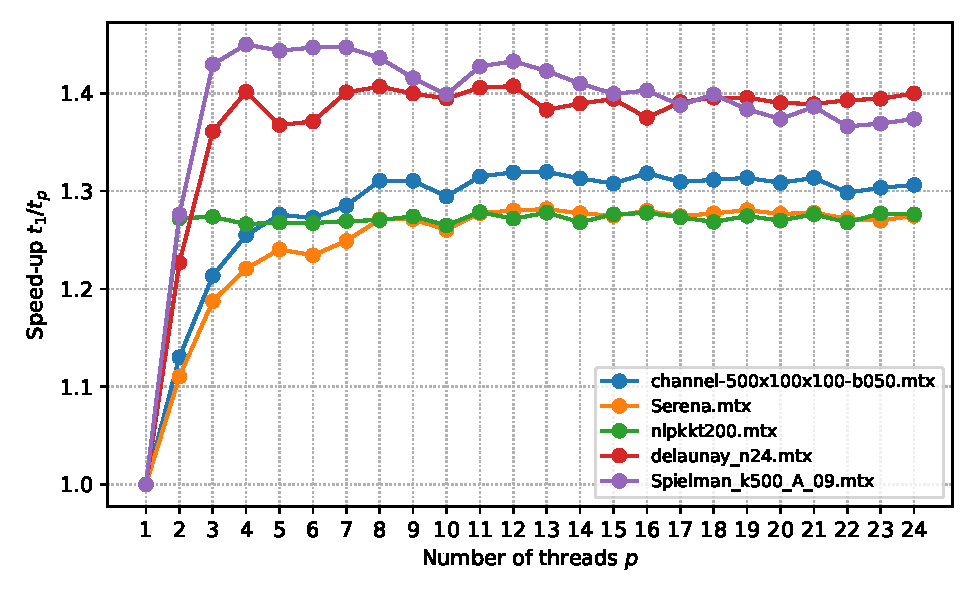
\includegraphics[width=\linewidth]{report/figures/results/speedup_t_tasks_ms_top5.pdf}
  \caption{Strong–scaling of the task-based bi-block solver
           (five largest matrices, see
           Table \ref{tab:matrices_benchmarks}), executed on the compute-p1 node of DelftBlue.}
  \label{fig:parallel_speedup_task}
\end{figure}

\begin{figure}[htb]
  \centering
  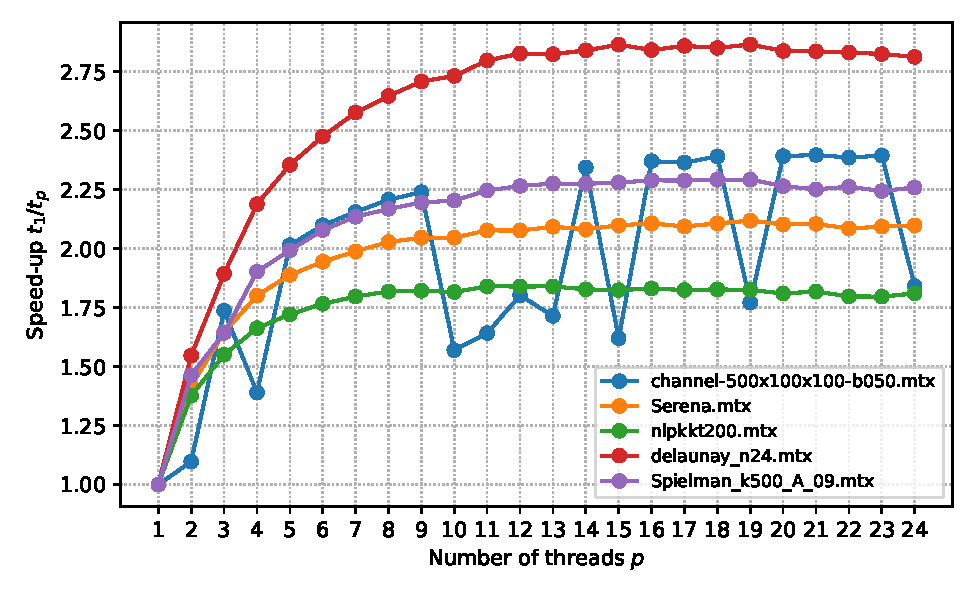
\includegraphics[width=\linewidth]{report/figures/results/speedup_t_trilinos_ms_top5.pdf}
  \caption{Strong–scaling of the Kokkos-Kernels
           \texttt{sptrsv} implementation for the same matrices and
           hardware as in Fig. \ref{fig:parallel_speedup_task}.}
  \label{fig:parallel_speedup_kokkos}
\end{figure}

For the task–graph solver
(Fig. \ref{fig:parallel_speedup_task}) the speed-up ranges from
$1.28$ ( \texttt{Serena} ) to $1.45$
( \texttt{Spielman\_k500\_A\_09.mtx} ).  
Across all cases the curve flattens once $p\gtrsim6$ because
\emph{Phase 2} (see Section \ref{chap:meth_task_sched}) becomes the critical path and thus further threads can only
steal leftover provisional tasks whose contribution to total run time
is already marginal.

Kokkos-Kernels exhibits a larger head-room
(Fig. \ref{fig:parallel_speedup_kokkos}):
$S(24)$ varies between $1.75$ and $2.8$
and saturation is only reached around $p=16$.

A notable outlier is \texttt{channel-500x100x100-b050.mtx}, whose speed-up curve alternates between two distinct plateaus, an indication that Kokkos-Kernels may toggle between two internal solve strategies for this matrix.

Intel MKL is not included in the scaling plots because
\texttt{mkl\_sparse\_trsv} is a sequential kernel
and therefore provides no meaningful parallel speed-up curve.
Its single-thread timing will be used as a performance baseline in the next sections.

%====================================================================
\subsection{Run-Time Versus Problem Size}
\label{sec:results_runtime_vs_nnz}
%--------------------------------------------------------------------
Figure \ref{fig:runtime_vs_nnz_grid} juxtaposes the
solve times of the three solvers (Intel MKL, the task–graph implementation, and the
Kokkos–Kernels reference) against the matrix size
(measured by the number of non-zeros $N_{nz}$).
Each panel fixes the thread count $p\in\{1,6,12,24\}$;
the horizontal axis is shared so that slopes can be compared
directly. All measurements were obtained on the compute-p1 node of DelftBlue (Table \ref{tab:platforms}).

At $p=1$ (upper-left panel) MKL unsurprisingly delivers the
fastest solves; its algorithmic overhead is modest and
the code is heavily optimised for serial performance.
The task solver follows the same trend
but incurs a higher constant cost because symbolic
permutation and task management are executed on the critical
path.  Kokkos–Kernels is the slowest method for most matrices, showing a larger overhead.

When additional threads become available
($p=6$, $12$, $24$) the curves of the parallel solvers turn
downwards, while the single–threaded MKL line stays in place.
For the task solver the improvement is noticeable up to
about six threads and then flattens, in line with the
strong–scaling results discussed later in
Section \ref{sec:results_speedup}.
Kokkos–Kernels continues to shorten run-time up to
$p\approx 16$ and then levels off where the turning point depends
on the matrix structure.

A final observation from Figure \ref{fig:runtime_vs_nnz_grid} is that
for small matrices ($N_{nz} \lesssim 10^{7}$) the
one-threaded Intel~MKL routine is consistently the fastest of the
three solvers even when parallel resources are available.
The higher constant overheads of the task graph (task creation) and of Kokkos-Kernels (kernel-handle initialisation,
generic data structures) outweigh their potential to exploit additional
threads.  Only when the matrix exceeds roughly ten million non-zeros does the
parallel execution of the task solver or Kokkos become beneficial
relative to MKL’s highly tuned serial path.

Because absolute run-times obscure the relative gains, and because the performance of the solvers lie very close together,
the next section converts these measurements into
speed-up curves,
which better expose algorithmic scalability.

\begin{figure}
  \centering
  \begin{subfigure}[t]{0.49\linewidth}
    \centering
    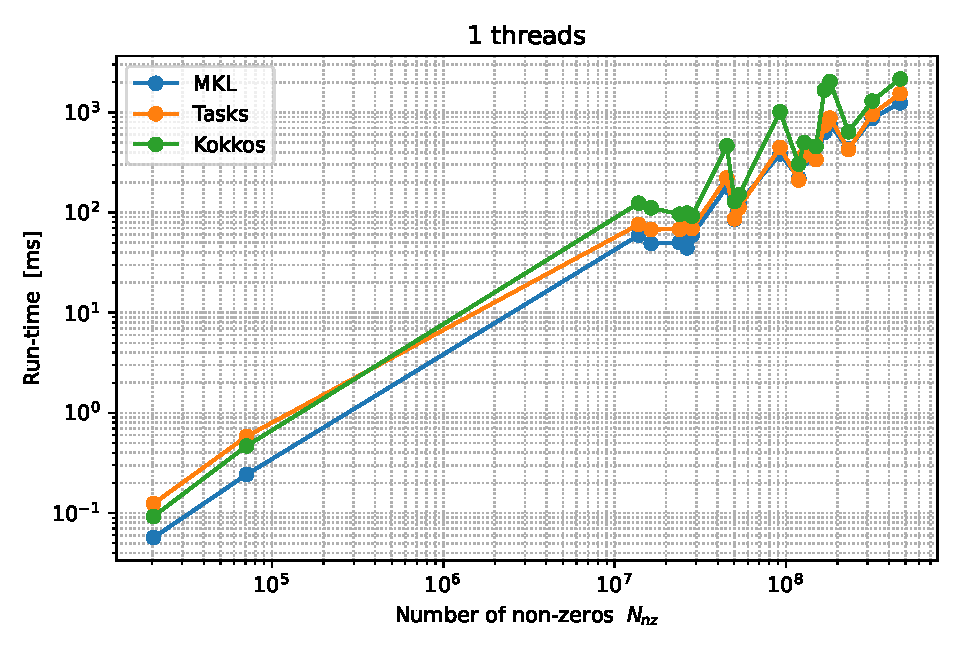
\includegraphics[width=\linewidth]{report/figures/results/runtime_vs_nnz_1.pdf}
    \caption{$p=1$ thread}
  \end{subfigure}
  %
  \begin{subfigure}[t]{0.49\linewidth}
    \centering
    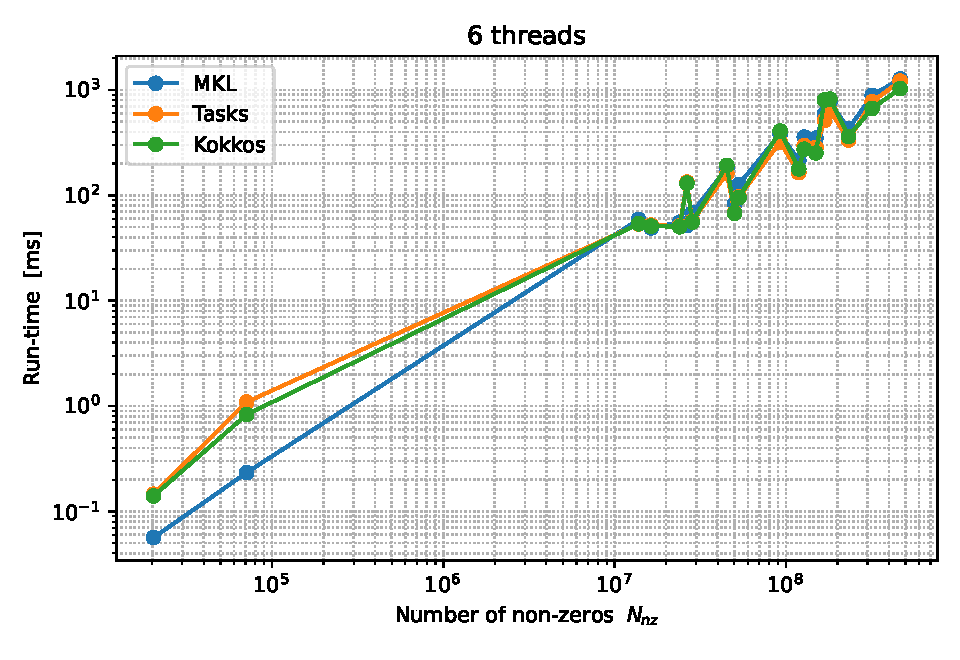
\includegraphics[width=\linewidth]{report/figures/results/runtime_vs_nnz_6.pdf}
    \caption{$p=6$ threads}
  \end{subfigure}
  \\
  \begin{subfigure}[t]{0.49\linewidth}
    \centering
    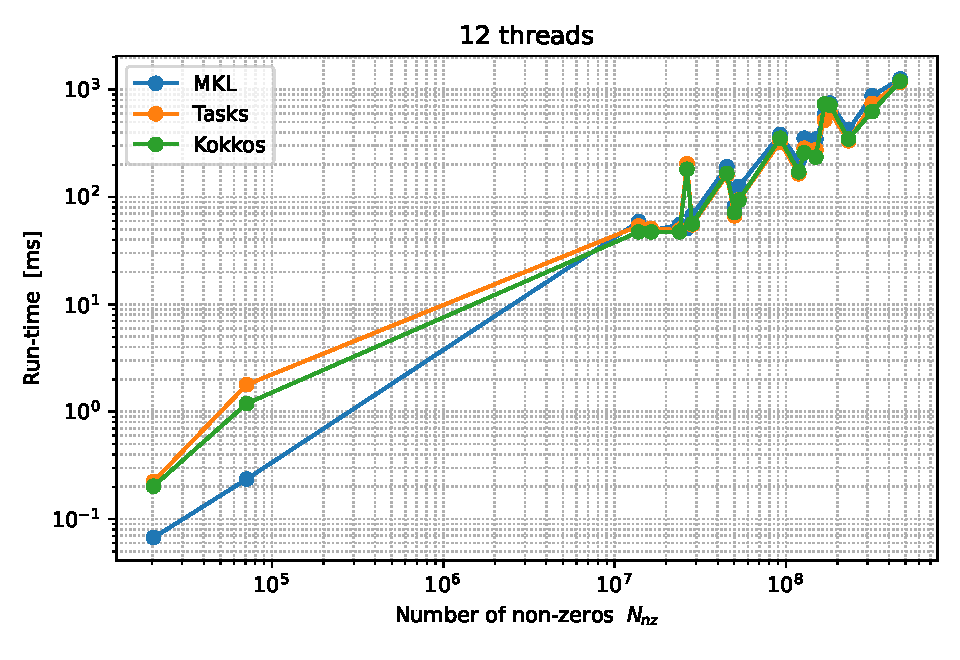
\includegraphics[width=\linewidth]{report/figures/results/runtime_vs_nnz_12.pdf}
    \caption{$p=12$ threads}
  \end{subfigure}
  %
  \begin{subfigure}[t]{0.49\linewidth}
    \centering
    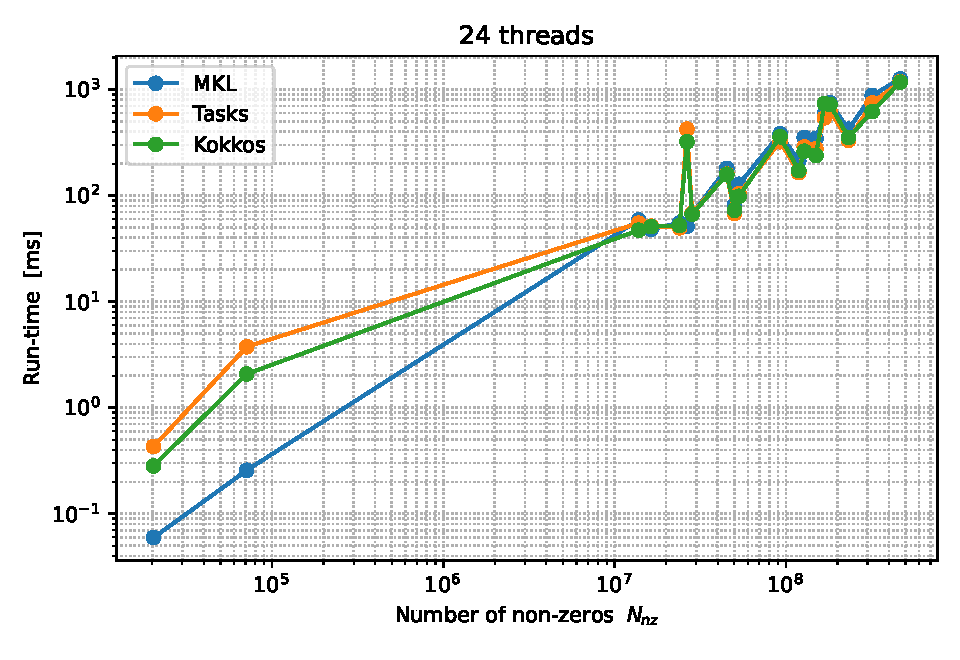
\includegraphics[width=\linewidth]{report/figures/results/runtime_vs_nnz_24.pdf}
    \caption{$p=24$ threads}
  \end{subfigure}
  \caption{Run-time versus problem size for the three solvers.
           Each line connects matrices in ascending $N_{nz}$ order and both axes use logarithmic scales. Measurements performed on the compute-p1 node of DelftBlue.}
  \label{fig:runtime_vs_nnz_grid}
\end{figure}


%====================================================================
\subsection{Cross–Solver Comparison}
\label{sec:results_rel_speedup}
%---------------------------------------------------------------
Figure \ref{fig:rel_speedup_mkl_tasks} shows the ratio
$t_{\mathrm{MKL}}/t_{\text{tasks}}$ while
Figure \ref{fig:rel_speedup_kokkos_tasks} reports
$t_{\mathrm{Kokkos}}/t_{\text{tasks}}$.
Each curve corresponds to a fixed thread count
$p\in\{1,6,12,24\}$ and is plotted over the non–zero count
of the test matrices. Measurements were once again performed on an exclusive compute-p1 node on DelftBlue (Table \ref{tab:platforms}).

Because Intel MKL’s triangular kernel is single-threaded, the ratio
$t_{\mathrm{MKL}}/t_{\text{tasks}}$ grows with $p$ making
our implementation up to an order of magnitude faster at
$p=24$.
For $p=1$ the Intel MKL solver is in almost all cases the faster method as should be expected.

In Figure \ref{fig:rel_speedup_mkl_tasks} there is one very notable outlier to the general performance trend, this turns out to be caused by matrix \texttt{Ship\_003}.
\texttt{Ship\_003} is the only test matrix that is symmetric positive-definite in its original form and therefore a direct Cholesky candidate. Its factor $L$ develops large, nearly dense super-nodes and RACE collapses these into just a few bulky diagonal blocks, leaving virtually no task-level parallelism. Our two–pass task kernel still incurs its bookkeeping overhead, but with little memory latency to overlap, this cost dominates the run time.
Conversely, \texttt{mkl\_sparse\_d\_trsv} detects the dense structure and switches to a vectorised dense micro-kernel that streams efficiently through contiguous data, even in a single thread.
Hence \texttt{Ship\_003} falls far below the general speed-up trend: MKL outperforms the task solver and additional threads cannot close the gap.
The anomaly delineates the solver’s scope: it excels on irregular, latency-dominated triangular factors, but its edge disappears when the factor resembles a dense panel already handled efficiently by a tuned serial routine.
\begin{figure}
    \centering
    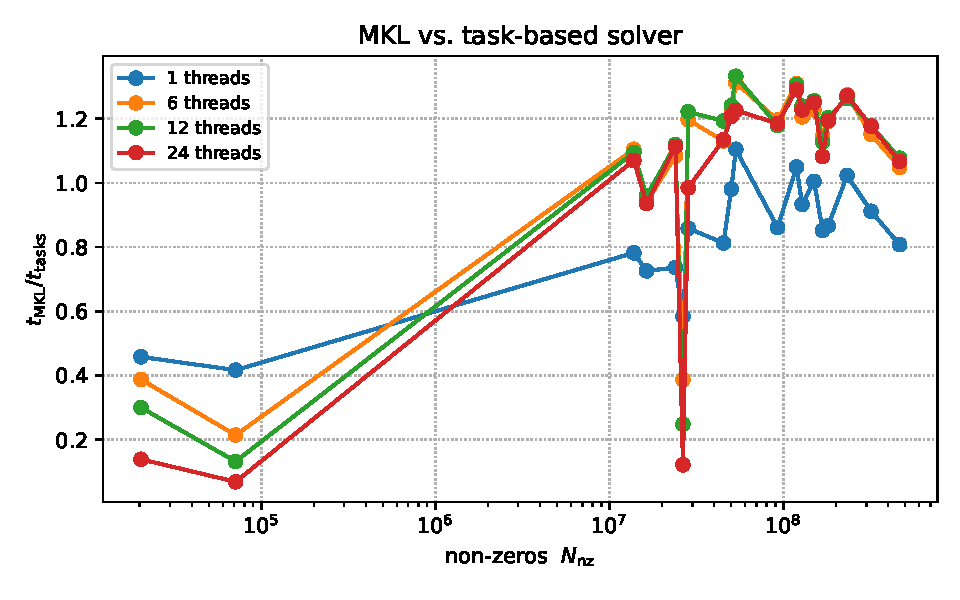
\includegraphics[width=1\linewidth]{report//figures//results/rel_speedup_mkl_vs_tasks.pdf}
    \caption{Relative speed-up $\displaystyle\frac{t_{\text{MKL}}}{t_{\text{tasks}}}$.
Points above 1 indicate that the task-based solver outperforms Intel MKL and
points below 1 indicate the opposite.  Results are shown for
$p = 1,\,6,\,12,$ and 24 threads, with matrices ordered by increasing
$\mathrm{nnz}$.}
    \label{fig:rel_speedup_mkl_tasks}
\end{figure}

The curves in Figure \ref{fig:rel_speedup_kokkos_tasks}
lie much closer to the horizontal axis,
staying between $0.75$ and $1.5$ for almost the entire size range when more then one thread is used.
This confirms that after the strong-scaling “plateau” of
Figure \ref{fig:parallel_speedup_task} is reached both
parallel algorithms become memory-bound and therefore deliver
very similar absolute performance.
The apparent advantage of Kokkos at $p\ge 12$ must therefore be read
with caution: it reflects the fact that our method saturates a few
threads earlier and subsequently shows little change, whereas the
Kokkos implementation continues to shorten its run time until about
$p\approx16{-}18$.
When the arithmetic workload is tiny (leftmost data points) the Kokkos
solver is clearly faster for $p \geq1$.

\begin{figure}
    \centering
    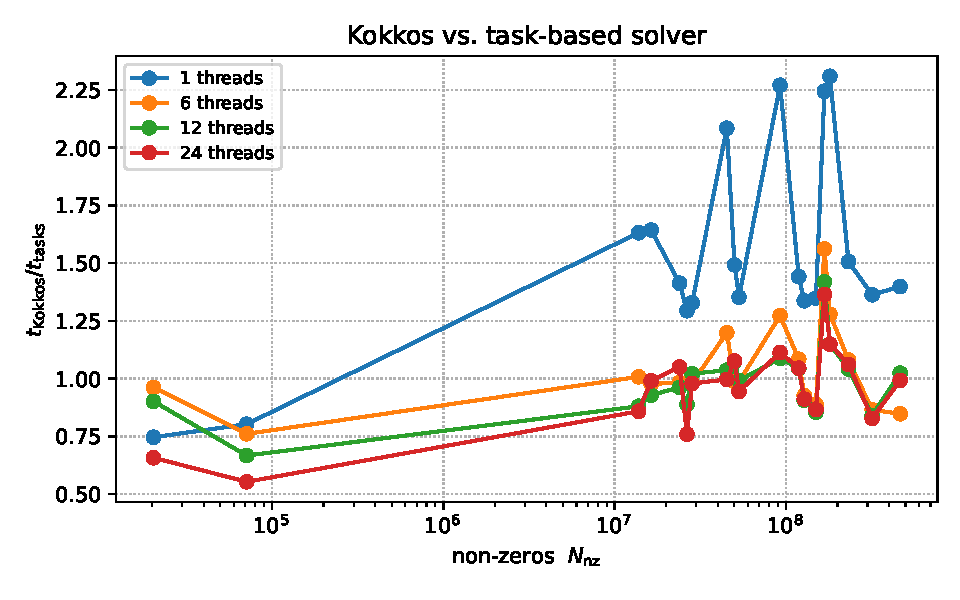
\includegraphics[width=1\linewidth]{report//figures//results/rel_speedup_kokkos_vs_tasks.pdf}
    \caption{Relative speed-up $\displaystyle\frac{t_{\text{Kokkos}}}{t_{\text{tasks}}}$.
Values above 1 mean the task-based solver is faster than the Kokkos-Kernels
implementation, while values below 1 favour Kokkos.}
    \label{fig:rel_speedup_kokkos_tasks}
\end{figure}

The two ratios underline that speed-up is a relative metric:
although Kokkos attains larger strong-scaling factors
(Figure \ref{fig:parallel_speedup_kokkos}),
its advantage in wall-clock time shrinks once both solvers are limited
by memory bandwidth.
Put differently, the task‐graph formulation reaches the memory-bound
regime earlier, so its speed-up curve becomes flat
before Kokkos has exhausted all available cores.
For large matrices and $p\ge12$ the two implementations therefore
exhibit virtually identical run times.

Across the large-matrix test set no single solver dominates
universally: for some inputs the task-based bi-block method is faster,
for others the Kokkos implementation wins.
The relative ranking therefore depends on the individual sparsity
pattern rather than on matrix size alone.

%---------------------------------------------------------------------------
\subsection{LIKWID Results}
\label{sec:results:cache-reuse}
All LIKWID measurements were taken on the DelftBlue compute-p2 node (\ref{tab:platforms}).
The region of our solver was instrumented with the \textit{L3}, \textit{L2/L2CACHE}
and \textit{DATA} event groups.
The \textit{MEM} group is unavailable on this
platform because current LIKWID versions cannot program the Intel Sapphire Rapids
integrated-memory-controller, so the counters \texttt{CAS\_COUNT\_RD/WR}
return 0. Consequently, the analysis below focuses on the on-chip hierarchy only.

LIKWID was used to measure the difference in performance of the task-based model implemented with OpenMP in Section \ref{sec:impl_tasks}, before the affinity clause was added to the OpenMP directives. 
To interpret the cache behaviour we restrict the discussion to a single
matrix that cannot reside in any on-chip cache and therefore
stresses the reuse mechanisms most: \texttt{nlpkkt200} (see Table \ref{tab:matrices_benchmarks}).
After the $A^3$ expansion and triangular extraction the factor
is sure to not fit in the cache memory of \textit{DelftBlue}.


With the LIKWID \texttt{L3}, \texttt{L2CACHE} and \texttt{DATA} groups
the triangular solve of our task kernel (16 threads) reports

$$
\mathrm{L3\;loads}=7.1\;\text{GB}, \quad
\mathrm{L3\;miss\;ratio}=12\%, \qquad
\mathrm{L2\;miss\;ratio}=91\%.
$$

The missing \texttt{MEM} group on Sapphire Rapids prevents
direct DRAM-traffic measurements; nonetheless the figures are
consistent with an in-LLC working set.
Almost every line requested by a core is absent from its private L2,
but nine out of ten are satisfied in the shared LLC, so only
$\approx 0.85\;\text{GB}$ of the 7.1 GB finally spill to memory.

A {\small $\sim$90 \%} L2 miss rate means that most provisional and
correction tasks run on different cores:
the provisional pass of block~$i$ brings
$L_i$ and $x_i$ into its private cache, the correction pass is then stolen by
another worker, and the data are fetched again from LLC.
This behaviour confirms the suspicion that the default
work-stealing policy weakens the intended producer–consumer affinity.
When the same thread executed both phases in quick succession one would
expect up to 50 \% L2 hits, because an entire $L_i$ ($\le$2 MiB)
fits into a single private cache.

In Section~\ref{sec:impl_tasks_aff} the \texttt{affinity} clause was
added to the OpenMP task directives to keep each correction task on the
same core that had just produced its matching provisional result,
thereby preserving the block data in the private~L2 cache.  Owing to
time constraints in the final week of the project, a second LIKWID
counter study could not be performed; only wall-clock timings were
recorded.

Those timings are nevertheless decisive.  For every matrix and for all
thread counts $p\in\{1,2,3,6,9,12\}$ the version with the
\texttt{affinity} hint outperforms the earlier non-affine
implementation.  Figure~\ref{fig:speedup_non_aff_aff} plots the ratio
$$
  \text{speed-up}_{\mathrm{aff}}=\frac{t_{\text{no-affinity}}}{t_{\text{affinity}}},
$$
so values above $1$ indicate a benefit from affinity scheduling.  The
average improvement ranges from $\sim1.1\times$ for single-thread
runs—where no scheduling decisions are necessary—up to almost
$\sim2 \times$ for nine threads.  This confirms the intuition from
Section \ref{sec:impl_tasks_aff}: suppressing work-stealing along the
tightly coupled correction chain leads to markedly better cache-line
reuse and shorter overall solve time, even though the
\texttt{affinity} clause is merely a hint and the OpenMP runtime may, in
principle, choose a different mapping.
\begin{figure}
    \centering
    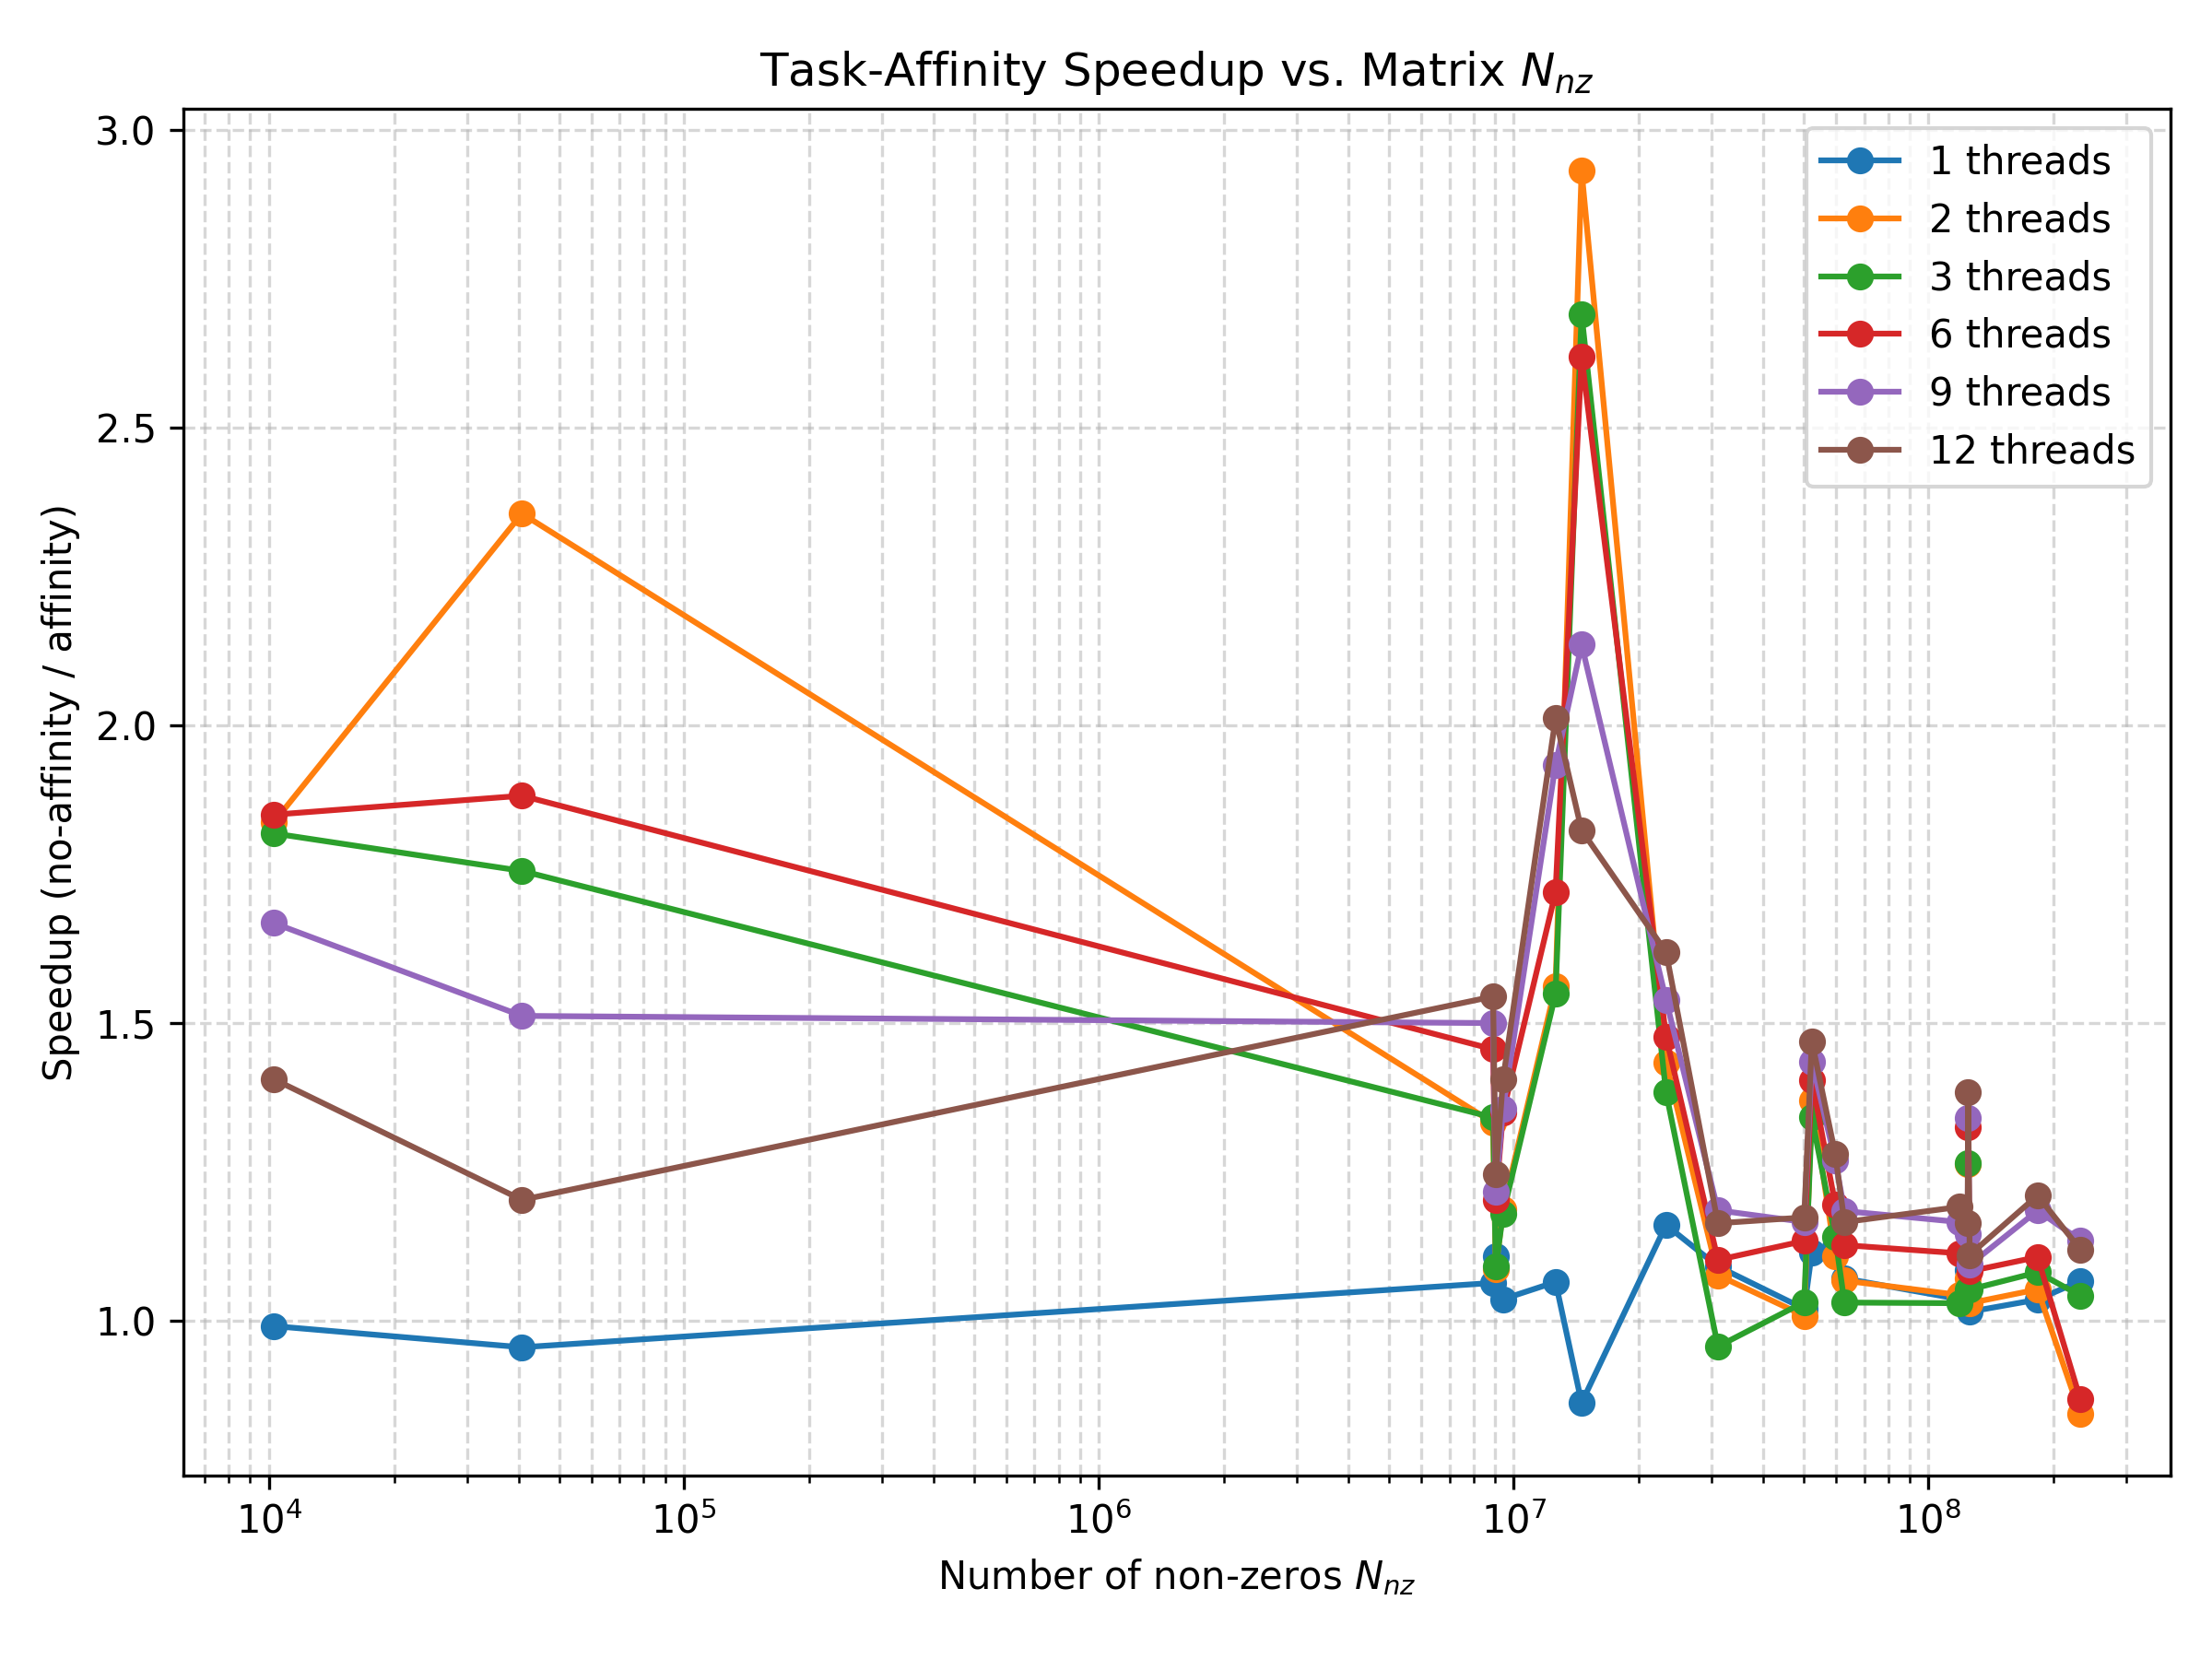
\includegraphics[width=1\linewidth]{relative_speedup_affinity_non_aff.png}
    \caption{Relative speed-up between the task based solver when implemented with and without affinity clause. Speed-up is given by solve time of implementation without affinity divided by the implementation with affinity for p $\in \{1,2,3,6,9,12 \}$ threads.}
    \label{fig:speedup_non_aff_aff}
\end{figure}
%---------------------------------------------------------------------------

\section{Reproducibility and Data Availability}
\label{sec:results_data}
All raw CSV measurements, plotting scripts, and the exact solver
sources that produced the figures of this chapter are publicly
available at \url{https://github.com/IdsRehorst/Bachelor-Thesis-Ids-Rehorst}.
The repository’s \texttt{tests/} directory contains
\texttt{benchmark\_\(<p>\).csv} files – one per thread count – that hold  
the median run time of every matrix and solver variant,  
ready for independent analysis or alternative visualisations.
